% --------------------------------------------------------------
% This is all preamble stuff that you don't have to worry about.
% Head down to where it says "Start here"
% --------------------------------------------------------------
 
\documentclass[11pt]{article}
 
\usepackage[margin=0.7in]{geometry} 
\usepackage{amsmath,amssymb}
\usepackage{hyperref}
\usepackage{amsfonts}
\usepackage{graphicx}
\usepackage{subfig}

\hypersetup{
  colorlinks   = true, %Colours links instead of ugly boxes
  urlcolor     = blue, %Colour for external hyperlinks
  linkcolor    = blue, %Colour of internal links
  citecolor   = red %Colour of citations
}

\usepackage{algorithm2e}


\usepackage{tcolorbox}
\setcounter{section}{-1}
\graphicspath{ {./img/} }

 
\newtheorem{theorem}{Satz}
\newtheorem{acknowledgement}[theorem]{Acknowledgement}
\newtheorem{axiom}[theorem]{Axiom}
\newtheorem{case}[theorem]{Case}
\newtheorem{claim}[theorem]{Claim}
\newtheorem{conclusion}[theorem]{Conclusion}
\newtheorem{condition}[theorem]{Condition}
\newtheorem{conjecture}[theorem]{Conjecture}
\newtheorem{corollary}[theorem]{Corollary}
\newtheorem{criterion}[theorem]{Criterion}
\newtheorem{definition}[theorem]{Definition}
\newtheorem{example}[theorem]{Example}
\newtheorem{exercise}[theorem]{Exercise}
\newtheorem{lemma}[theorem]{Lemma}
\newtheorem{notation}[theorem]{Notation}
\newtheorem{problem}[theorem]{Problem}
\newtheorem{proposition}[theorem]{Proposition}
\newtheorem{remark}[theorem]{Remark}
\newtheorem{solution}[theorem]{Solution}
\newtheorem{summary}[theorem]{Summary}
\newenvironment{proof}[1][Beweis]{\textbf{#1.} }{\ \rule{0.5em}{0.5em}}
\begin{document}
 
% --------------------------------------------------------------
%                         Start here
% --------------------------------------------------------------
 
\title{Principles of Computer Graphics - Summary}%replace X with the appropriate number
\author{Andy Tràn}
 
\maketitle %shows the current date of the Zusammenfassung

This will be a very personalised summary for me to use to study for the course Principles of Computer Graphics (CSCI3260). It might be complete, it might not be, it will probably not be. For questions you can refer to \href{mailto:andtran@ethz.ch}{andtran@ethz.ch}. This summary is based of the lecture notes and should be used as a supplement to the lectures. 

\tableofcontents

\newpage

\section{Important organizational stuff}
\begin{itemize}
    \item \href{mailto:pheng@cse.cuhk.edu.hk}{pheng@cse.cuhk.edu.hk}, office hours: Thursday 2:30 PM - 4:30 PM, SHB 929
    \item \textbf{Lecture hours:}  Tuesday 10:30 am - 12:15 pm, Thursday 11:30 am - 12:15 PM
    \item \textbf{Tutorial hours}: Monday 3:30 pm - 4:15 pm, Thursday 5:30 pm - 6:15 pm 
    \item \textbf{Reference book}: Fundamentals of Computer Graphics by Peter Shirley (not necessary), OpenGL Programming Guide
    \item \textbf{Course}: Consists of three parts: introduction, basics in graphics, more about graphics 
    \item \textbf{Grading}: (2) programming assignments 0.25, course project 0.20, mid-term exam 0.25, final exam 0.30
    \item \textbf{Release}: Assignment 1 - release 12/9, deadline 02/10, assignment 2 - release 3/10, deadline 30/10, course project - release 31/10, deadline 27/11, mid-term exam 18/10 10:30 - 12:15
\end{itemize}
\section{Lecture 1 - 06/09/2022: Introduction, Display and Colour}
\subsection{Display and Colour}
Lecture Outline
\begin{itemize}
    \item Display Devices and Basic Terminologies
    \item Frame Buffer (Memory to Display)
    \item Color Space: RGB, CMY, HSV, YIQ, CIE YZ
    \item ALpha Channel and Double Buffering
\end{itemize}

\subsubsection{Display Devices}
\textbf{Mechanism:}  shoot electrons with varying energy through vertical and horizontal deflectors to hit spot on screen, phosphors on screen jump to excited state when hit by electrons, emit monochromatic light when they drop to rest state
\newline
\textbf{Random scan/Vector scan:}  give instruction and follow instruction
\newline
\textbf{Raster scan:}  you go in a line and activate a line, and you turn each line on, where each spot on the screen is called a pixel. You shoot the gun, at the end of the line you turn it off and go back to the start, which is called \textbf{retrace}. There is a difference between horizontal and vertical retrace, horizontal is per line, vertical for each following line.
\newline
\textbf{Interlacing:} trick to get less flicker out of fixed signal bandwidth, it's like doubling the framerate, for example let's say we have 30Hz, we send two signals but each with a time difference between each other. For example to line 0 we send at 0 and 1, line 1 we send at 2 and 3. 
Result: doubling the perceived the framerate, without costing more bandwidth
\newline
Flat-Panel displays, two classes
\begin{itemize}
    \item \textbf{Nonemissive displays}: LCD (optical effects to split light)
    \item \textbf{Emissive display}: field emission display (FED), light-emitting diode (LED), organic light-emitting diode (OLED). Which is more power efficient
\end{itemize}
\noindent
On LCD: we block light instead of emitting the correct light.
\newline
FED: thousands of micro-electron guns

\subsubsection{3D Displays overview}
Two human visual cues used 
\begin{itemize}
    \item Stereopsis: seeing 2 slightly different images in each eye
    \item Motion Parallax: seeing slighty different images as you move around
\end{itemize}
\noindent
Terms used:
\begin{itemize}
    \item Stereoscopic: difference image to each eye, viewer must wear special glasses
    \item Autostereoscopic: different image to each eye, does not require special glasses
    \item Multi-view: different images depending on viewer's position
\end{itemize}
Note: Multi-view can be combined with used in combination of the others
\newline
\subsubsection{Stereoscopic and Autostereoscopic displays}
\begin{itemize}
    \item Stereoscopic displays (common): two approaches
     \begin{enumerate}
        \item using circularly polarized glasses (like in cinemas)
        \item using active shutter glasses (requires batteries, for example 3D TVs)
    \end{enumerate}
    \item Autostereoscopic displays: two approaches
    \begin{enumerate}
        \item Lenticular lens: bright but blurry, old
        \item Parallax barriers, darker but sharper, like Nintendo 3DS
    \end{enumerate}
\end{itemize}
\noindent
Downside of Autostereoscopic displays: usually limited to 1 or a very few viewers, and narrow sweet spot for viewing 3D.

\subsubsection{Multi-view displays}
Usually enabled by tracking the person's head.

\subsection{Frame Buffer}
Graphical storage (memory) and transformation hardware for digital images. We consider computer images as digital, we want to quantify a space into units (pixels).

\subsubsection{Greyscale/Monochrome Frame Buffer}
\begin{itemize}
    \item Intensity of the raster scan beam is modulated according to the contents of a frame buffer
    \item Each element of the frame buffer is associated with a single pixel on the screen
\end{itemize}
Each marker corresponds to a pixel on the computer screen, remember rasterizing from the beginning of this lecture

\noindent
Note: digital to analog converted (DAC)

\subsubsection{Resolution}
Determined by 
\begin{itemize}
    \item number of scan lines
    \item number of pixels per scan line
    \item number of bits per pixel
\end{itemize}

\subsubsection{Colours}

\begin{itemize} 
    \item 1 bit: B or W, 8 bit: 0 pure black to 255 pure white, with colours in between. To have true colour we need 8 bit per RGB
    \item To produce colours we mix intensities of each colour, to have a full spectrum we need a monitor which supports 256 voltages for each colour, the description of each colour in frame buffer memory is called \textbf{channel}. The term \textbf{truecolour (24 bits)} is for systems which the frame buffer stores the values for each channel (3 channels for RGB) 
    \item \textbf{Color table}: for few bits per pixel, we have to map non-displayable colours to displayable ones. We can remap color table entries in software. 
\end{itemize}

\subsubsection{Look Up Tables (LUT)}
Pseudo color: assign computed values systematically to a gray or color spectrum to indicate differences, for example height, speed, etc. 

\subsection{Color Space}
\begin{enumerate}
    \item RGB: additive color space, used for displays
    \item CMY: subtractive color space, used for printing
    \item HSV: (H circular, S distance from axis, V brightness), corresponds to artistic concepts of tint, shade, and tone
    \item YIQ: (Y luminance, I orange-cyan hue, Q green-magenta hue), exploits properties of the visual system, used in TV broadcasting
    \item XYZ system: defined in terms of three color matching functions  
\end{enumerate}

\begin{definition}[Gamut] 
    device's range of reproducible color
\end{definition}

\subsection{Alpha Channel and Double Buffering}
\subsubsection{Alpha Channel}
\textbf{Idea:}  we store one color per pixel, but we get hard edges. So we introduce an alpha channel next to the RGB channel, to blend with the lower layers to smoothen it out. Can be regarded as \textbf{1 - transparency} or \textbf{opacity}. 

\begin{example}[Blending]
    We have a source and destination image, we can overlay them and the alpha value denotes of how much percentage we see each image when we overlay them
\end{example}

\subsubsection{Image Matting} 
What part of the image we want to keep, using a mask.

\subsection{Double Buffering}
\begin{problem}
    what happens when we write to the frame buffer while it's being displayed?
\end{problem}
\begin{solution}[Double-buffering]
    \begin{enumerate}
        \item Render to the the back buffer and swap when rendering is done
        \item Double the memory
    \end{enumerate}
\end{solution}

\section{Lecture 2 - 08/09/2022: Useful 2D and 3D mathematics}
\subsection{Coordinate Systems}
\subsubsection{2D Cartesian Reference Frames}
There are two ways of using this system: (a) starting at the lower-left screen corner, (b) starting at the upper-left screen corner. 

\subsubsection{Polar Coordinates in the XY plane}
We start from a center, with a radial distance \textbf{r} and the angular displacement $\theta$   from the horizontal   
\newline
We can convert it to the cartesian system: $x = r cos \theta$ and $y = r sin \theta$ 
\newline
To polar system: $r = \sqrt{x^2 + y^2}$ and $ \theta = tan^{-1}(\frac{y}{x})$    
\newline
\textbf{Definition}: $\theta = \frac{s}{r}$, where $\theta$ is the angle subtended by the circular arc of length s and r
\newline
We know: $P = \frac{2\pi r}{r} = 2\pi$, total distance around P
\subsubsection{3D cartesian reference frames}
\textbf{Right-handed system}: Take your right hand, palm towards you, thumb (positive x direction) to the right, index finger up (positive y direction), middle finger towards you (positive z direction). Yes, the back of you is positive z.
\newline 
\textbf{Left-handed system}: Like RHS, but this time away from you is positive z. (Think of how to use your hand to show this)
\newline
In OpenGL: right handed (common), DirectX free to choose   
\subsubsection{Cylindrical-coordinate System}
\begin{enumerate}
    \item The surface of constant r is a vertical cylinder
    \item The surface of constant $\theta$ is a vertical plane containing the Z-axis
    \item The surface of constant z is a horizontal plane parallel to the Cartesian XY plane
    \item Transformation from a cylindrical coordinate specification to a cartestian reference system 
\end{enumerate}

$X = r cos \theta $, $Y = r sin \theta$, $ Z = z$

\subsubsection{Spherical-coordinate system}
Which is like polar coordinate in 3D space, we have $P(r,\theta,\phi)$
\newline
it holds that $x = r cos \theta sin \phi$, $y= r sin \theta sin \phi$, $z r cos \zeta$    

\begin{definition}[Angles in 3D] We define it as $ \omega = \frac{A}{r^2}$, total area is $\frac{4\pi r^2}{r^2} = 4\pi$ 

    
\end{definition}

\subsection{Points and Vectors}
\textbf{2D vector}:  $V = P_2 - P_1 = (V_x, V_y)$, length is defined as $\sqrt{V_x^2 + V_y^2}$, angle is $\alpha = tan^{-1}(\frac{V_y}{V_x})$ 
\newline
\textbf{3D vector}: V is same as 2D but with one more value, length is defined equivalently with $V_z$. We have three direction angles %todo

We have the following rules
\begin{enumerate}
    \item Addition: $V_1 + V_2 = (V_{1x} + V_{2x}, V_{1y} + V_{2y}, V_{1z} + V_{2z})$
    \item Scalar multiplication: $aV = (aV_x, aV_y, aV_z)$
    \item Scalar product: $V_1 \cdot V_2 = |V_1||V_2|\cos \theta$, from there you can derive $\theta$    
    \item Normalization: $\frac{V}{|V|}$, so its own product is 1
    \item Perpendicular: $|A||B|\cos \theta = A \cdot B =
     \begin{cases}
        0 & \text{if } \theta = 90 deg\\
        > 0 & \text{if }\theta < 90 deg\\
        < 0 & \text{otherwise}
    \end{cases}$  
    \item Cross product of two 3D vectors: $V_1 \times V_2 = u |V_1||V_2|\sin \theta$, where u is the unit vector that is perpendicular to both $V_1$ and $V_2$ %TODO\
    \item Basis vectors: we can specify the coordinate axes in any reference frame with a set of vectors, one for each axis
\end{enumerate}

\section{Lecture 3 - 13/09/2022}
\textit{Continuation of previous lecture}
Properties of cross product
\newline
\begin{itemize}
    \item Anti-commutative: $V_1 \times V_2 = -(V_2 \times V_1)$
    \item Non-associative: $V_1 \times (V_2 \times V_3) \neq (V_1 \times V_2) \times V_3$
    \item Distributive: $V_1 \times (V_2 + V_3) = (V_1 \times V_2) + (V_1 \times V_3)$   
\end{itemize}

\subsection{Useful 2D mathematics}
\begin{enumerate}
    \item Distance from P to line AB: \begin{itemize}
        \item Find line direction: $v = (x_2 - x_1, y_2 - y_1) = (d_x , d_y)$
        \item Find normal of line by swapping elements in v: $ n = (-d_y, d_x) = (y_1 - y_2, x_2 - x_1)$ 
        \item Normalize n and v as $\hat{n}, \hat{v}$  
        \item Use dot product to find h and l: $h = |(P-A) \cdot \hat{n}$, $l = (P - A) \cdot \hat{v}$  
        \item Need to check l against length of AB
        \item If $l < 0$ or $l > |AB|$, compute point-point distance  
    \end{itemize}
    \item Line-Line intersection: \begin{itemize}
        \item Express as parametric forms: $AB: (x_1, y_1) + t_{AB} (x_2 - x_1, y_2 - y_1)$ , $CD: (x_3, y_3) + t_{AB} (x_4 - x_3, y_4 - y_3)$ and set them both equal
        \item If no solution, that meas they are parallel
        \item Substitute back to the parametric form
    \end{itemize}
    \item Which-side test: given a point and a line, 
    Calculate %TODO
    \item Area of arbritrary polygons: polygon area $\frac{1}{2} \sum det ...$ %TODO
    \item Inside-outside test: \begin{itemize}
        \item Method 1: repeat the which-side test for each edge in order (only works for convex polygons)
        \item Method 2:Odd-intersection count, side =  $\begin{cases}
            \text{outside}, & number \equiv_2 0\\
            \text{inside}, & \text{otherwise}
        \end{cases}$
    \end{itemize}
    \item Linear Interpolation %TODO
    \item Barycentric coordinate: by means of area ratios %TODO
    \item Spherical linear interpolation %TODO
    \item Normal of a triangle %TODO
    \item Approximate normal at a vertex (vertex normal vs face normal): average the face normals of neighboring faces    
\end{enumerate}

\subsection{sth} %TODO
Properties
\begin{itemize}
    \item No fixed points under translation: all points move
    \item Multiple translations are order-independent, since addition is commutative 
\end{itemize}

\subsubsection{2D scaling}
Properties
\begin{itemize}
    \item Origin fixed: $x' = 0$ if $x=0$
    \item Order independent: $x'' = x' \cdot S_x' = x \cdot S_x \cdot S_x\  = x \cdot S_x' \cdot S_x$   
\end{itemize}
Single out \textit{arbitrary fixed point scaling} at $(x_0, y_0)$ as follows:
\begin{align*}
    x' &= x\cdot S_X + (1-S_x)x_0 \\
    y' &= y\cdot S_y  + (1-S_y)y_0
\end{align*} 

Rotate by $\theta$:
\begin{align*}
    x'&= r \cos (\theta + \phi) = r \cos \phi \cos \theta - r \sin \phi \sin \theta\\
    y' &= r \sin (\theta + \phi) = r \sin \phi \cos \theta + r \cos \phi \sin \theta
\end{align*} 
Multiple 2D rotations are order-independent
Fixed-point: origin dependent
\subsubsection{Other 2D transformations}
\begin{itemize}
    \item Reflection (about X/Y - axis): not equal to a rotation, except when reflecting over x and y, then it's a rotation
\end{itemize}
2D shearing: order dependent %TODO

\subsection{Matrix operations} %TODO need to check how to write matrixes quickly and easily slide 50

%TODO blablalba

\subsubsection{Homogenous representations}
\begin{enumerate}
    \item Translation cannot be represented using $2 x 2$  matrices and homogenous coordinates help
    \item We are left-multiplying the matrix on the vector/point 
\end{enumerate}



%FIX LECTURE 3
\section{REAL Lecture 3: Hierarchical Model}
\subsection*{Lecture Outline}
\begin{enumerate}
    \item Graphics Primitives: Points, Lines and Triangles
    \item Data structure: vertex list and index list
    \item Hierarchical Structure
    \item View-world or Modelview transformations
    \item Basic scenegraph concept
\end{enumerate}

\subsection{Graphics Primitives: Points, Lines and Triangles}

\begin{itemize}
    \item \textbf{Idea:} It's all about \textbf{coordinates} and \textbf{connectivity}
    \item \textbf{Meaning:} wireframe and meshes are built up by points, lines, or triangles. We call this \textbf{tesselation/triangulation}
    \item \textbf{Most efficient input type for rendering polygons:}  \textbf{Triangle strip} or \textbf{triangle fan}. The differences between the two is the following, triangle strip is a set of triangles which share vertices (can share different vertices), while triangle fan has one \textbf{(!)} shared center. 
\end{itemize}

%TODO: include img of TS and TF, they are in the ./img/folder   

\subsection{Data structure: vertex list and index list}
We have two kinds of data strucutres, namely vertex lists and index lists. 
\begin{itemize}
    \item \textbf{Vertex list:} you store all the vertex coordinates in one array \begin{itemize}
        \item Benefit: sequential memory access
        \item Negative: very likely to have duplicated vertices in the array, waste of storage
    \end{itemize}
    \item \textbf{Index list/Indexed Face Set:} we have two arrays, one called the \textbf{face list}. That one contains all the polygons and the corresponding vertices. While the \textbf{vertex list} contains the coordinates for each vertex. \begin{itemize}
        \item Benefit: reuse vertices and keeps a compact vertex list
        \item Bad: random memory accesses which lead to cache misses
    \end{itemize}
\end{itemize}

\textit{Note:} (1) triangle strip can be implemented on either data structure, (2) in some APIs these data structures are built in, (3) indexing can start with 0 or 1.

\subsection{Hierarchical structure}
A scene is composed of the multiple objects, which are composed of subjects as well. We can create a hierarchical model and break it down. Each objects has its own polygon list and associated vertex list.
\subsection{View-world or Modelview transformations}
\begin{itemize}
    \item \textbf{Idea:}  we model objects in a model space, which is pretty dumbed down in a cartesian matter where we start from the origin. (\textbf{Model space}) This usually doesn't reflect the reality and we want to model it to the common world (\textbf{World space}) and then to our eyes perspective (\textbf{Eye perspective}). 
    \item \textbf{Example:}  we create a moon in the object space, we put it in the sky, and then we look at it. 
    \item \textbf{Concrete:} An object is defined as $P_{obj} = (x,y,z)^T$ to get it into the world coordinates we need to transform it, namely $M_{obj2world} \times P_obj$ and to get the eye coordinates, $M_{world2eye}\times M_{obj2world} \times P_obj$.
    \textbf{Note:} Since we usually don't care about the steps inbetween, we usually merge $M_{obj2world}$ and $M_{world2eye}$ into one matrix called the \textbf{modelview/viewworld} $M_{modelview}$.
\end{itemize}


Notes about the modelview Matrix $M_{modelview}$:
\begin{itemize}
    \item OpenGL puts the eye-point at the origin looking towards the negative z-axis
    \item OpenGL is a state machine: it has an internal memory storage for the modelview matrix
    \item When calling transformation operations, the kernel constructs a matrix for the transform and right multiplies it with its internal modelview matrix.
\end{itemize} %TODO: explain what point 3 does exactly?

%TODO: show to illustration from the slides, we have mv_steps.png to import
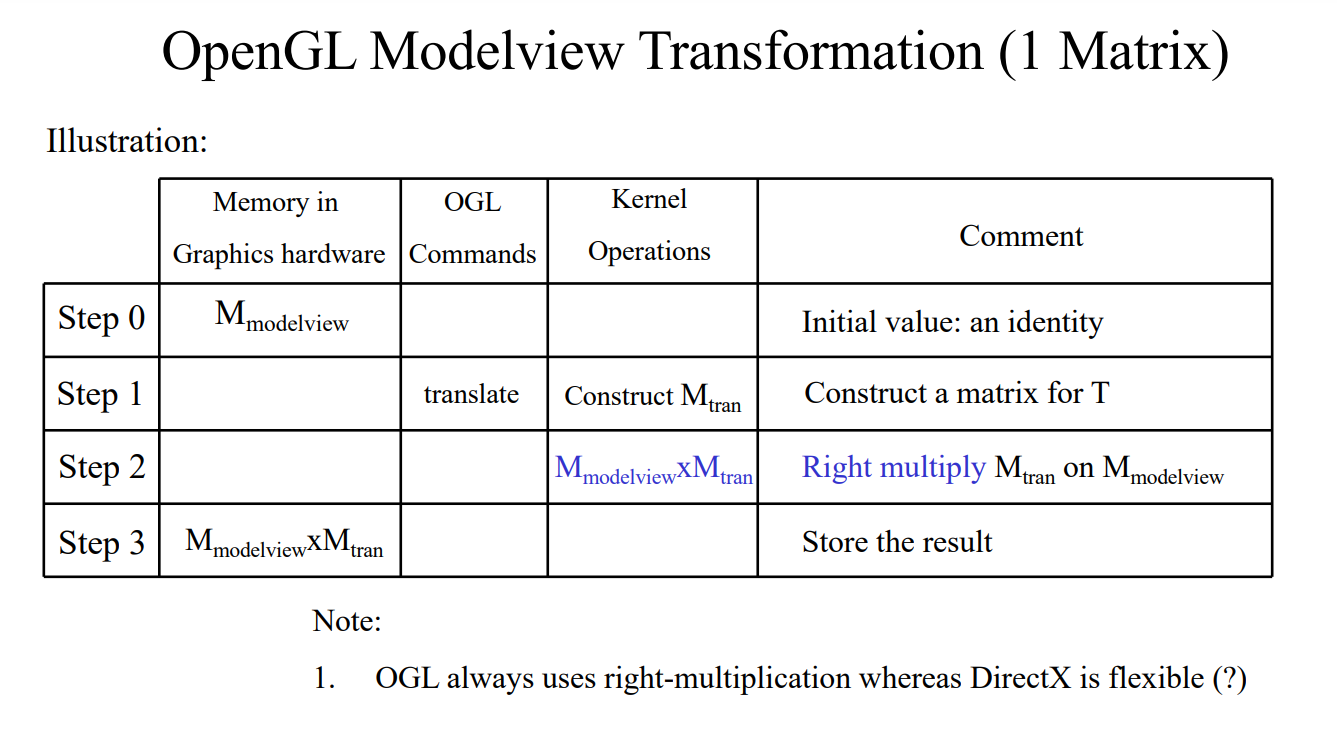
\includegraphics[scale=.5]{mv_steps.png}
 
\subsection{Basic scenegraph concept}
\begin{itemize}
    \item Organize the whole model hiearchy as a tree structure
    \item Examples of language who do that: VRML, OpenSG
\end{itemize}

How does this work exactly? We have group nodes, who associate nodes into hierarchies, leaf nodes, who contain all the descriptive data of objects in the virtual world used to render them.

\subsubsection*{Avoid Modeling Glitches}
\begin{enumerate}
    \item Avoid T-Join \begin{itemize}
        \item Problem: we have edges which sometimes don't touch due to computation and rounding errors of floats
        \item Solution: we break a triangle into two triangles.
    \end{itemize}
    \item Avoid overlapping polygons in your model \begin{itemize}
        \item Problem: overlapping triangles give flipping colors (\textbf{z fighting})
        \item Solution: create another triangle for the overlapping area, or turn off depth test when drawing the next triangle
    \end{itemize}
    
    
\end{enumerate}
 

\section{Lecture 4: Interactive 3D Control}
\subsection*{Lecture Outline}
\begin{enumerate}
    \item Interactive Control Concept
    \item Interactive Translation relative to screen
    \item Interactive rotation: rolling ball
\end{enumerate}

\subsection{Interactive Control Concept}
\begin{itemize}
    \item \textbf{Idea:} we use the mouse as an input device for 3D viewing control
    \item \textbf{Approach:} by modifying the (base) 4x4 Modelview matrix incrementally accordingly to the mouse motion, we can control our 3D viewing interactively. 
\end{itemize}

\textbf{Normal Modelview Transformation Equation:}  assume the modelview matrix is affine. In particular, it has translation, rotation and scaling only. If so we can write the Modelview transformation like this:

\[
    \begin{bmatrix} x_{eye}\\ y_{eye} \\ z_{eye} \\ 1 \end{bmatrix} = \begin{bmatrix} m_{11} & m_{12} & m_{13} & T_x \\ 
        m_{21} & m_{22} & m_{23} & T_y \\
        m_{31} & m_{32} & m_{33} & T_y \\
        0 & 0 & 0 & 1\end{bmatrix} \begin{bmatrix} x_{world} \\ y_{world} \\ z_{world} \\ 1 \end{bmatrix} 
.\]


\subsection{Interactive Translation relative to screen}
Left-Multiply a translation matrix to the existing modelview. We can have a screen-aligned translation, since we don't need to use the fixed point rule for translations.

%TODO: show OpenGL implementation, all in slides

\subsection{Interactive rotation: rolling ball}
If we want to rotate our existing modelview, one of the most common mistakes being made is left-multiplying the rotation matrix to our modelview. We need to apply the \textbf{fixed point rule}
\begin{enumerate}
    \item Undo the translation $(T_x, T_y, T_z)$ in the modelview matrix
    \item Left-multiply the rotation matrix
    \item Redo the translation $(T_x, T_y, T_z)$ 
\end{enumerate}
\noindent
Now we need to construct the rotation matrix, to map our 2D mouse motion to a 3D rotation.
\begin{itemize}
    \item \textbf{Method:}  rolling ball
    \item \textbf{Idea:} imagine the object is inside a glass ball of radius r.
    \item To construct the rotation matrix: \begin{enumerate}
        \item Put the mouse motion in an XY-eye space: (dx, dy, 0)
        \item Axis of rotation perpendicular to the motion vector: (-dy, dx, 0)
        \item Angle of rotation relative to motion vector length: $\sqrt{dx^2 + dy^2}$ 
    \end{enumerate}

    %TODO: include graphic of OGL implementation
    
\end{itemize}

\section{Lecture 5: Cameras, Projections, and Clipping}
\subsection*{Lecture Outline}
\begin{enumerate}
    \item Pin-hole camera
    \item Family of Projections
    \item Parallel Projection
    \item Perspective Projection
    \item OpenGL Projection Model: 4x4 projection matrix
    \item Clipping and Perspective Division
\end{enumerate}

\subsection{Pin-hole camera}
\begin{itemize}
    \item How does a pin-hole camera work: we have a (small) hole to focus all light in an area. The object goes through an barrier and is displayed on film. The image is always inverted
    \item \textbf{Advantages:} easy to simulate, everything is in focus
    \item \textbf{Disadvantages: } needs a bright scene (long exposure), everything is in focus (not realistic in photography)  
\end{itemize}

There is also second method, namely a camera with lens
\begin{itemize}
    \item How does a camera with a lens work: an object goes through a lens and falls on a focal point. The distance between lens and camera is called focal length. You can compare this to an eye where the eye is the lens and it falls on cones. 
    \item \textbf{Advantages: } no need to have a bright scene, not everything is in focus (more realistic in photography)
    \item \textbf{Disadvantages: } need more programming to simulate, not everything is in focus  
\end{itemize}

Now, we don't care about cameras that much obviously, how does it work in programming or even OpenGL?
Namely, the OpenGL viewpoint acts as a virtual camera, to define a camera we need the following
\begin{enumerate}
    \item Viewpoint (what is in the middle of our view)
    \item View direction
    \item Field of view (in degrees)
    \item Film size 
    \item Projection plane
\end{enumerate}

Viewing requires three elements:
\begin{itemize}
    \item Objects to be viewed, e.g. whatever you are taking a picture of (1), input geometry (2)
    \item A viewer with a projection surface, e.g. the camera (1), OpenGL camera (2)
    \item A projection from the objects to the viewing surface, e.g. defined by the lens, map 3D objects to the 2D surface (1), OpenGL projection matrix (2)
\end{itemize}
(1) being real life, (2) OpenGL

\subsubsection*{Planar Geometric Projections}
\begin{itemize}
    \item Standard projections are assumed to be onto a single plane (2D)
    \item There are two kinds of projections \begin{enumerate}
        \item Perspective projection: all rays converge at a single point (center of projection)
        \item Orthographic projection: all rays are parallel
    \end{enumerate}
\end{itemize}

\noindent We need coordinate systems to render geometry objects, in the following way:
\newline
$
\text{Object space} \stackrel{Linear trans}{\to} \text{World space} \stackrel{Linear trans}{\to} \text{Eye/Camera space} \stackrel{Non-lin trans}{\to} \text{Screen space} \stackrel{raster.}{\to} \text{Raster space} $

\subsubsection*{Object space}
\begin{itemize}
    \item Most natural coordinate space
    \item Local coordinate system, local to the object
    \item Other name: modeling coordinate system
\end{itemize}

\subsubsection*{World space}
\begin{itemize}
    \item A coordinate system that is shared by all objects in the modeled scene
\end{itemize}

\subsubsection*{Eye/Camera space}
\begin{itemize}
    \item The coordinate system with the eye or the center of projection as its origin
    \item A space in which the viewing volume is established
    \item Facilitates clipping (removing out-of-view objects)
\end{itemize}

\subsubsection*{Screen space}
\begin{itemize}
    \item Transformation to screen space is a process that describes how light rays reach our eyes
    \item Screen space is defined to act within a closed volume called the viewing frustum
\end{itemize}

\begin{itemize}
    \item Viewing coordinates system, $[x_v, y_v, z_v]$ describes 3D objects with respect to a viewer
    \item A viewing plane is set up perpendicular to $z_v$ and aligned with $(x_v, y_v)$
    \item To set up a viewing plane we need
    \begin{itemize}
        \item $P = (P_x, P_y, P_z)$ the point where the camera is located
        \item L, the point to look at 
        \item V, the view-up vector whose projection onto the view-plane is directed up
    \end{itemize}
\end{itemize}

To form a viewing coordinate system we can calculate the following, $Z_v = \frac{P-L}{|P-L|}, X_v = \frac{V\times Z_v}{|V\times Z_v|}, Y_v = Z_v \times X_v$. The transformation matrix M from world-coordinate into viewing-coordinates is defined as 
\[
M = \begin{bmatrix} x_v^x & x_v^x & x_v^x & 0 \\ y_v^x & y_v^x & y_v^x & 0 \\ z_v^x & z_v^x & z_v^x & 0 \\ 0 & 0 & 0 & 1  \end{bmatrix}  \begin{bmatrix} 1 & 0 & 0 & -P_x\\ 0 & 1 & 0 & -P_y \\ 0 & 0 & 1 & -P_z\\ 0 & 0 & 0 & 1 \end{bmatrix} = R\cdot T 
.\]  

\subsubsection*{3D Projection}
\begin{itemize}
    \item We model in 3D, but final display on the monitor is 2D
    \item Projection refers to the process of projecting the 3D world into 2D, the visualizing of it.
    \item Two major types of projection: perspective, like the eye; orthogonal projection, preserve length after projection, used in CAD systems
\end{itemize}

What is a projection:
Squeezing a higher dimension into a lower dimension, where in graphics usually 3D to 2D.


\subsection{Family of Projections}
%TODO insert image of family of projections
\subsubsection*{Parallel vs perspective projections}
\begin{itemize}
    \item In 3D we map points from 3-space to the projection plane (PP) along projection lines emanating from the center of projection
    \item The center of projection (COP) is exactly the same as the pinhole in a pinhole camera
\end{itemize}%TODO insert image of page 23 lecture 5



\subsection{Parallel Projections}
We can specify direction of projection (DOP) because all projections lines are parallel
\begin{enumerate}
    \item Oblique projection (DOP not perpendicular to PP) 
    \item Orthographic projection (DOP perpendicular to PP)
\end{enumerate}

\subsubsection*{Oblique Projection (Parallel)}
Like shearing the geometry along PP, two standards of oblique projection:
\begin{enumerate}
    \item Cavalier projection \begin{enumerate}
        \item DOP makes 45 degree angle with PP
        \item Does not foresherten lines perpendicular to PP
        \item Preserves length
    \end{enumerate}
    \item Cabinet projection \begin{enumerate}
        \item DOP makes 63.4 degrees angle with PP
        \item Foreshorten lines perpendicular to PP by one-half (called Chinese Perspective)
    \end{enumerate} 
\end{enumerate}

\subsubsection*{Orthographic Projection (parallel)}
\begin{enumerate}
    \item Orthogonal Projection \begin{itemize}
        \item DOP align with object's X, Y, or Z-axis
        \item implementation: just throw away one of the dimensions (set to 0)
        \item side, top/plan, or front views
    \end{itemize}
    \item Axonometric projection \begin{itemize}
        \item arbitrary DOP, not parallel to world X, Y, nor Z-axis
        \item special case: isometric (exactly 120 degrees)
    \end{itemize}
\end{enumerate}

Properties of parallel projection: 
\begin{itemize}
    \item Not realistic looking
    \item Good for exact measurements, remember for CAD!
    \item Kind of affine transformations, parallel lines remain parallel, angles not preserved
\end{itemize}

\subsection{Perspective Projection}
\begin{itemize}
    \item COP is at finite distance to the PP, so the further away an object is, the smaller it is
    \item How we see the nature
\end{itemize}

\subsubsection*{Vanishing points}
\begin{itemize}
    \item There exist infinitely many vanishing points
    \item There can be up to three principal vanishing points (on the axes)
    \item Perspective projections are categorized by the number of principal vanishing points, equal to the number of principal axes intersected by the viewing plane
    \item Most commonly used: one-point and two-points perspective
\end{itemize}

In perspective transformation, parallel lines appear to converge to a single point (easy to see if we have squares and draw parallel lines.)\newline
\textbf{Vanishing point: } points at which parallel lines on PP  
%TODO: there is a summary of projections in page 35

\subsubsection*{View Frustum: the visible "volume" }
%TODO: idk what this is, have to look it up

\subsection{OpenGL Projection Matrix: 4x4 projection matrix}
OpenGL projection settings:
\begin{enumerate}
    \item Eye/camera position:
    \item Viewing direction
    \item View-up direction
    \item Viewing region (viewing frustum)
    \item Visible depth range
\end{enumerate}

\subsubsection*{Orthographic Projection in OpenGL}
We can use the method \textit{glOrtho(l,r,b,t,n,f)} or \textit{gluOrtho2D(l,r,b,t)}. Where they stand for left, right, bottom, top, neara, far. In gluOrtho2D, near is set to 0, far to 1.

\subsubsection*{Perspective Concept in OpenGL}
Let's say a point is proejcted onto the projection plane, the x and y coordinates are scaled. We can compute it using following: $x_c = -\frac{x}{z}, y_c = - \frac{y}{z}$. For $z_c$, I can't find it, but a smaller $z_c$ means a closer clip coordinate from the eye.    

\subsection{Clipping and Perspective Division}
Perspective division: $x' = x_\frac{c}{w_c}, y' = \frac{y_c}{w_c}, z' = \frac{z_c}{w_c}$ 

%TODO: missing a few info about clippign...

\subsubsection*{Viewport transformation}
glViewport(x,y,width, height) is a command, to define the rectangle where the image is mapped in window pixel coordinates. 
We need to pay attention the aspect ratio!




\section{Lecture 6: Clipping}
\subsection*{Lecture contents}
\begin{itemize}
    \item Purpose: eliminate portions of objects outside the viewing Frustum
    \item View frustum: boundaries of the image plane projected in 3D, a near and far clipping plane
\end{itemize}
%TODO: include graph page 2

Reasons to use clipping
\begin{itemize}
    \item Avoid degeneracies: we don't draw stuff behind the eye, and avoid division and overflow
    \item Efficiency: we don't care about stuff we don't see
    \item Prevent unnecessary rasterization (which is expensive)
\end{itemize}

What will come later is culling. The name says enough, if a part is partially in and outside we need to clip, if it's completely outside we need to cull. The final image must be no different than if we didn't do any of this!

There are different strategies
\begin{itemize}
    \item Don't clip, lol
    \item Clip during rasterization
    \item Analytical clipping: alter input geometry
\end{itemize}

\subsubsection*{Point Clipping}
Given a point (x,y,z) we have to determine whether it's in our viewing volume, which is the easiest.
Namely, our view frustum consists of 6 planes, we have to test again each plane. If $H\cdot p < 0$, we reject. Where a plane is defined by $Ax + By + Cz +D  = 0 $, and $H = (A,B,C,D)$, we assume $D = 1$ for now and $p = (a,b,c,1)$   

\subsubsection*{Line Clipping}
Idea is similar, let's say we have a segment PQ, we check the following for each plane.

\begin{itemize}
    \item If $H\cdot P > 0$ and $ H\cdot q < 0$, then clip q to plane
    \item If $H\cdot p < 0$ and $H \cdot q > 0$, then clip p to plane
    \item If $H\cdot p > 0$ and $H \cdot q > 0$, pass through
    \item If $H\cdot p < 0$ and $H \cdot q < 0$, clipped out         
\end{itemize}

Also, to see the intersection point we can use the maths from one of the first lectures to get it.

There is also another mathematical way, namely computing the sidedness of each vertex with respect to each bounding plane and combine using logical AND. 

Cohen-Sutherland Line Clipping Algorithm:
\begin{enumerate}
    \item First, outcode of end-points pairs are checked for trivial acceptance
    \item If the line cannot be trivially accepted, region checks are done trivial rejection
    \item If line cannot be trivially accepted or rejected, subdivide so that one or both segments can be discarded
    \item These three steps are performed iteratively until what remains can be trivially accepted or rejected
\end{enumerate}

%TODO: more detail later

\subsubsection*{Polygon Clipping}
Polygon clipping is symmetric, even when concave or convex. In the most naive case we make $N*m$ intersection and link all segments. We could walk along the boundary CCW and compute intersection points where they enter and leave the window.
\newline
Walking rules: 
\begin{itemize}
    \item Out-to-in pair: record clipped point and follow polygon boundary ccw
    \item In-to-out pair: record clipped point and follow window boundary ccw
\end{itemize}

Using this we know which part falls within the window.

\section{Lecture 7: Rasterization and Anti-aliasing}
\subsection*{Lecture outline}
\begin{enumerate}
    \item Introduction to rasterization
    \item Rasterization algorithms
    \item Introduction to anti-aliasing
    \item Anti-aliasing concepts
    \item Anti-aliasing in graphics hardware
\end{enumerate}

\subsection{Introduction to rasterization}
Idea is, we have polygons, with information like color, depth, etc. We want to display them on our display (on the raster), so we need a method to do it, since our screen is only finite.
So how does it work:
\begin{enumerate}
    \item Select pixels on the screen, that best cover the 2D continuous geometry
    \item Then interpolate the per-vertex information for each pixel
    \item Geometries include: points, lines, triangles, bitmap, etc.
    \item Hardware (part of graphics hardware) is called rasterizer
\end{enumerate}

\subsection{Rasterization algorithms}
\subsubsection*{Points}
There are two ways, namely
\begin{itemize}
    \item Draw a square (non-antialiased)
    \item Draw a circle (antialiased)
\end{itemize}

Shortly, why we can draw circle, is to make it not look as rough, for example for lines we want to smoothen it out since we don't have an infinite amount of pixels.

\subsubsection*{Line drawing}
We need to approximate the mathematical lines if we want to draw a line: $y = mx + b$, which we learned to calculate in school.

%TODO: I dont really understand this, have to look at it again.


\subsubsection*{Triangle}
We subdive polygons into triangles (we can always do this), and now we just have to rasterize the triangles.
This can be done efficiently, because of:
\begin{enumerate}
    \item Scan line coherence: long horizontal stretches of the same fill value
    \item Edge coherence: easy to use line algorithm to computer next scan line's end points
\end{enumerate}

%TODO: i actually dont really understand this LOL

\subsection{Introduction to anti-aliasing}
\subsection{Anti-aliasing concepts}
\subsection{Anti-aliasing in grahics hardware}


\section{Lecture 8: Hidden Surface Removal}
\subsection*{Lecture Outline}
\begin{enumerate}
    \item Introduction Hidden Surface Removal
    \item Method 1: Ray Casting
    \item Method 2: Z Buffer Method
    \item Method 3: Back face culling
    \item Method 4: Potentially Visible Set (PVS)
    \item Hidden Surface Removal in OGL
\end{enumerate}


\subsection{Introduction to Hidden Surface Removal}
When we have multiple 3D objects, it's possible we don't see every part, since they could be hidden somewhere. Computationally it's expensive to still render them, and just better to remove them alas \textit{hidden surface removal/elimination}.

There are multiple methods on how to achieve it, for example object order and image order.
\subsubsection*{Object Order vs image order}
\begin{itemize}
    \item Object order: Each 3D object is considered and drawn once, we could draw same pixels multiple times if they overlap, for example Z-buffer
    \item Image order: Each pixel is considered once, so we draw one object and move on, we need to compute relationships between objects, for example Ray Casting
\end{itemize}

\subsubsection*{Sort first vs Sort last}
\begin{itemize}
    \item Sort first: find the depth-based ordering and draw from back to front, for example Painter's algorithm
    \item Sort last: sort implicitly as more information becomes available, for example Z-buffer
\end{itemize}

\subsection{Ray Casting}
The projection plane (PP) is partitioned into pixels to match screen resolution. \begin{itemize}
    \item For each pixel $p_i$, construct ray (projector) from COP through PP at that pixel and into scene
    \item Intersect the ray with every object in the scene, color the pixel according to the object with the closest intersection 
\end{itemize}

\subsubsection*{Implementation}
We have to parameterize the ray \[
R(t) = (1-t)c + tp_i
.\] 
\begin{itemize}
    \item If a ray intersects some object $O_i$, get parameter t such that first intersection with $O_i$ occurs at $R(t_i)$
    \item We have to find out which object owns the pixel 
\end{itemize}

More detail later in the course


\subsection{Z-Buffer method}
Idea is to have an additional channel in memory for pixel depth, which is called depth-buffer or Z-buffer (remember from the righthand's rule, z-axis is into or away from the screen). When drawing a pixel, we compare the depth, only draw when it's closer\dots

\subsubsection*{Implementation}
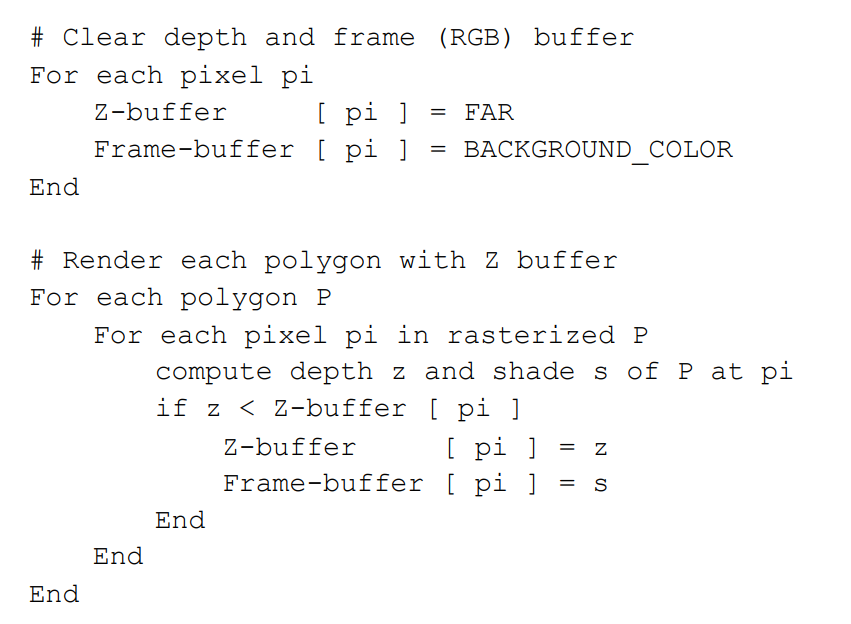
\includegraphics[scale=.8]{z_buff_implem}


\subsubsection*{Positives and Negatives}
\begin{itemize}
    \item Positive: \begin{itemize}
        \item Runtime is fast
        \item Simple to implement
    \end{itemize}
    \item Negative: \begin{itemize}
        \item Suffers from aliasing, e.g. z-fighting
        \item Cannot render transparency
    \end{itemize}
    
    
\end{itemize}

\subsection{Back face culling}
\begin{itemize}
    \item Used together with polygon-based algorithms, if we have solid objects, we don't need to draw polygons that are not in our view. So we can elimnate those (culling). 
    \item Can be used together with ray-casting and Z-buffer algorithms
    \item We need a normal vector (orthogonal to the plane), we check the angle between the viewer and the normal to some polygon. If it's between -90 degrees and 90 degrees $(\cos \theta \geq 0)$, then it's front facing.
    \item Or verify $N_p \cdot V$, where $N_p$ is the polygon normal, $V$ the line of sigh vector
    \item Hard to do for concave objects, that's why usually preprocessing step for Z-buffer or ray casting    
\end{itemize}

\subsection{Potentially visible set (PVS)}
\begin{itemize}
    \item Acceleration technique
    \item Data structure (usually pre-computed) that saves what parts of the region is always visible from within the region
    \item Divide into regions and precompute the objects
    \item Advantage: good speed up
    \item Disadvantage: extra memory, preprocessing time, doesn't allow dynamic scenes
\end{itemize}


\subsection{Hidden Surface Removal in OGL}
Three related modules:
\begin{enumerate}
    \item View Frustum Clipping, remove objects outside view
    \item Back-face culling
    \item Depth-buffering
    \item (Or Ray casting must be implented yourself)
\end{enumerate}

\subsubsection*{Back-Face Culling in OGL}
\begin{itemize}
    \item Done before rasterization step
    \item OGL functions: glEnable(GL\_CULL\_FACE) (or disable, which is standard); glFrontFace(mode) specify which is the front face; glCullFace(mode), which side to cull.
\end{itemize}

\subsubsection*{Depth Buffering}
\begin{itemize}
    \item Request depth buffer when creating a window, e.g. glutInitDisplayMode(...| GL\_DEPTH)
    \item Always clear depth buffer before rendering a screen again, with glClear and glClearDepth
    \item Enable depth test, glEnable(GL\_DEPTH\_TEST)
    \item glDepthFunc defines the test condition for pixel fragment, default and normal argument is GL\_LESS. All with smaller Z-value should pass
\end{itemize}


\end{document}